%label:"fig:ProductTorus"
%type:"figure"
%name:"product torus"
%caption:"Product Torus constructed via Lefschetz fibration"
%parent:"art_lefschetzExpanded"


        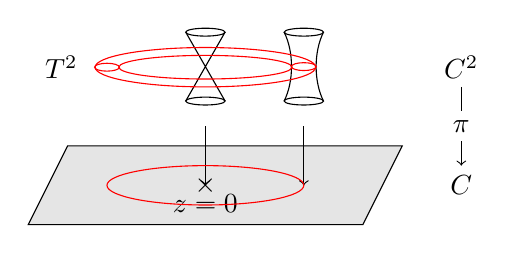
\begin{tikzpicture}[scale=.5]

\draw[fill=gray!20] (-2.5,2.5) -- (-3.5,0.5) -- (5,0.5) -- (6,2.5) -- cycle;
\begin{scope}[scale=0.5, shift={(6,3.78)}]
\draw  (-4,7) ellipse (1 and 0.2);
\draw  (-4,3.5) ellipse (1 and 0.2);
\draw (-5,7) -- (-3,3.5) (-5,3.5) -- (-3,7);
\end{scope}

\begin{scope}[scale=0.5,shift={(11,3.78)}]
\draw  (-4,7) ellipse (1 and 0.2);
\draw  (-4,3.5) ellipse (1 and 0.2);

\draw (-5,7) .. controls (-4.5,6) and (-4.5,4.5) .. (-5,3.5);
\draw (-3,7) .. controls (-3.5,6) and (-3.5,4.5) .. (-3,3.5);
\draw[red]  (-4,5.25) ellipse (0.63 and 0.2);
\end{scope}

\draw[->] (3.5,3) -- (3.5,1.5);
\draw[->](1,3) -- (1,1.5);
\node at (1,1.5) {$\times$};
\node[below] at (1,1.5) {$z=0$};


\node at (7.5,1.5) {$\mathbb C$};
\node at (7.5,4.5) {$\mathbb C^2$};
\draw[->] (7.5,4) -- (7.5,2);
\node[fill=white] at (7.5,3) {$\pi$};





\node[left] at (-2,4.5) {$T^2$};

\draw[red, scale=.5]  (-3,9) ellipse (0.63 and 0.2);

\draw[red]  (1,4.5) ellipse (2.8 and 0.5);
\draw[red]  (1,4.5) ellipse (2.2 and 0.3);
\draw[red]  (1,1.5) ellipse (2.5 and 0.5);

\end{tikzpicture}